\documentclass[10pt]{beamer}

\usetheme{Oxygen}
\usepackage{thumbpdf}
\usepackage{wasysym}
\usepackage{ucs}
\usepackage[utf8]{inputenc}
\usepackage{pgf,pgfarrows,pgfnodes,pgfautomata,pgfheaps,pgfshade}
\usepackage{verbatim}
\usepackage{tikzsymbols}

\usepackage{ragged2e} % maneja la alineación del documento
\usepackage[spanish]{babel} % Títulos en español
\usepackage[utf8]{inputenc}
%\usepackage[latin1]{inputenc} % Caracteres con acentos.
\usepackage{graphicx} % Soporte para gráficos
\usepackage[none]{hyphenat} % indica a LaTeX que no debe hacer partición de palabras
\usepackage[T1]{fontenc} % manejo de fuentes
\usepackage{array}
\usepackage{amsmath}
\usepackage{amssymb}
\usepackage{float}
%\usepackage{ra  gged2e}
\usepackage [all]{xy}
\usepackage{lmodern}
\usepackage{multirow}
\usepackage{multicol}
\usepackage{tikz}
\usepackage{listings}

\lstset{keywordstyle=\color{blue}, 
commentstyle=\color{gray!90}, 
basicstyle=\ttfamily\small, 
columns=fullflexible, 
breaklines=true,
linewidth=\textwidth, 
backgroundcolor=\color{gray!20}, 
basewidth={0.5em,0.4em}, 
literate={á}{{\'a}}1 {ñ}{{\~n}}1 {é}{{\'e}}1 {ó}{{\'o}}1 {º}{{\textordmasculine}}1, 
showstringspaces=false}



\setbeamersize{text margin left=9mm,text margin right=7mm} 


\pdfinfo
{
  /Title       (Maestría en Analítica e Inteligencia de Negocios)
  /Creator     (TeX)
  /Author      (Orlando Joaqui-Barandica)
}


\title{Maestría en Analítica e Inteligencia de Negocios}
\subtitle{Clase: Series de tiempo y pronóstico}
\author{PhD. St. Orlando Joaqui-Barandica} 
\institute{Universidad del Valle}
\date{2021}

\sloppy % Indica a LaTex que debe minimizar el corte de las palabras para pasar de una línea a otra
\justifying % justificar todo el documento


\begin{document}

\frame{\titlepage}


\begin{frame}
  \frametitle{Contenido}
  \tableofcontents[hidesubsections]
\end{frame}

\AtBeginSection[]
{
  \frame<handout:0>
  {
    \frametitle{Contenido}
    \tableofcontents[currentsection,hideallsubsections]
  }
}

    
\AtBeginSubsection[]
{
  \frame<handout:0>
  {
    \frametitle{Contenido}
    \tableofcontents[sectionstyle=show/hide,subsectionstyle=show/shaded/hide]
  }
}

\newcommand<>{\highlighton}[1]{%
  \alt#2{\structure{#1}}{{#1}}
}

\newcommand{\icon}[1]{\pgfimage[height=1em]{#1}}



%%%%%%%%%%%%%%%%%%%%%%%%%%%%%%%%%%%%%%%%%
%%%%%%%%%% Content starts here %%%%%%%%%%
%%%%%%%%%%%%%%%%%%%%%%%%%%%%%%%%%%%%%%%%%




\section{Métodos simples}

\begin{frame}[fragile]
\frametitle{Métodos simples de pronóstico}

Algunos métodos de pronóstico son extremadamente simples y sorprendentemente efectivos.

\vspace{4mm}

\begin{itemize}
\item \textbf{Método promedio}
\end{itemize}


los pronósticos de todos los valores futuros son iguales al promedio (o ``media'') de los datos históricos ${y_1, y_2, ..., y_T}$

\begin{equation}
\hat{y}_{T+h|T} = \bar{y} = \frac{y_1 + y_2 + ... + y_T}{T} 
\end{equation}


\lstset{language=r,label= ,caption= ,captionpos=b,numbers=none}
\begin{lstlisting}
meanf(y,h)

# y contiene la serie de tiempo
# h es el horizonte de pronóstico
\end{lstlisting}


\end{frame}


%%%%%%%%%%%%%%%%%%%%%%%%%%%%%%%%%%%%%%%%%%%%%%%%%%%%%%%%%%%%



\begin{frame}[fragile]
\frametitle{Métodos simples de pronóstico}


\begin{itemize}
\item \textbf{Método ingenuo}
\end{itemize}


Para pronósticos ingenuos, simplemente establecemos que todos los pronósticos sean el valor de la última observación. Es decir, Este método funciona notablemente bien para muchas series de tiempo económicas y financieras.

\begin{equation}
\hat{y}_{T+h|T} = y_T
\end{equation}


\lstset{language=r,label= ,caption= ,captionpos=b,numbers=none}
\begin{lstlisting}
naive(y,h)
rwf(y,h)  # Alternativa equivalente a naive
\end{lstlisting}

{\scriptsize
\textit{Debido a que un pronóstico ingenuo es óptimo cuando los datos siguen una caminata aleatoria (Ya veremos más adelante), estos también se denominan \highlighton{pronósticos de caminata aleatoria.}}
}

\end{frame}


%%%%%%%%%%%%%%%%%%%%%%%%%%%%%%%%%%%%%%%%%%%%%%%%%%%%%%%%%%%%



\begin{frame}[fragile]
\frametitle{Métodos simples de pronóstico}


\begin{itemize}
\item \textbf{Método ingenuo estacional}
\end{itemize}

Un método similar es útil para datos altamente estacionales. En este caso, establecemos que cada pronóstico sea igual al último valor observado de la misma estación del año (por ejemplo, el mismo mes del año anterior)

\begin{equation}
\hat{y}_{T+h|T} = y_{T+h-m(k-1)}
\end{equation}

dónde \textcolor{red}{$m$} es el periodo estacional y \textcolor{red}{$k$} es la parte entera de \textcolor{red}{$(h-1)/m$} (es decir, el número de años completos en el período de pronóstico anterior al tiempo \textcolor{red}{$T+h$})


\end{frame}


%%%%%%%%%%%%%%%%%%%%%%%%%%%%%%%%%%%%%%%%%%%%%%%%%%%%%%%%%%%%


\begin{frame}[fragile]
\frametitle{Métodos simples de pronóstico}


\begin{itemize}
\item \textbf{Método ingenuo estacional}
\end{itemize}

Esto parece más complicado de lo que realmente es. 

\vspace{4mm}

\begin{itemize}
\item Por ejemplo, con datos mensuales, el pronóstico para todos los valores futuros de febrero es igual al último valor observado en febrero. 
\item Con datos trimestrales, el pronóstico de todos los valores futuros de Q2 es igual al último valor observado de Q2 (donde Q2 significa el segundo trimestre). 
\item Reglas similares se aplican para otros meses y trimestres, y para otros períodos estacionales.
\end{itemize}


\lstset{language=r,label= ,caption= ,captionpos=b,numbers=none}
\begin{lstlisting}
snaive(y,h)
\end{lstlisting}



\end{frame}


%%%%%%%%%%%%%%%%%%%%%%%%%%%%%%%%%%%%%%%%%%%%%%%%%%%%%%%%%%%%



\begin{frame}[fragile]
\frametitle{Métodos simples de pronóstico}


\begin{itemize}
\item \textbf{Método con deriva}
\end{itemize}

\vspace{4mm}

Una variación del método ingenuo es permitir que los pronósticos \highlighton{aumenten} o \highlighton{disminuyan} con el tiempo, donde la cantidad de cambio a lo largo del tiempo (llamada deriva) se establece como el cambio promedio visto en los datos históricos.

\vspace{4mm}

Así, el pronóstico para el tiempo \textcolor{red}{T + h} está dado por:


\begin{equation}
\hat{y}_{T+h|T} = y_{T} + \frac{h}{T-1} \sum^{T}_{t=2} (y_t -y_{t-1}) = y_T + h\left( \frac{y_T - y_1}{T-1}\right) 
\end{equation}


\textit{Equivalente a dibujar una línea entre la primera y la última observación, y extrapolarla hacia el futuro.}

\lstset{language=r,label= ,caption= ,captionpos=b,numbers=none}
\begin{lstlisting}
rwf(y,h,drift = TRUE)
\end{lstlisting}



\end{frame}


%%%%%%%%%%%%%%%%%%%%%%%%%%%%%%%%%%%%%%%%%%%%%%%%%%%%%%%%%%%%



\begin{frame}[fragile]
\frametitle{Ejemplo}



\lstset{language=r,label= ,caption= ,captionpos=b,numbers=none}
\begin{lstlisting}
beer2 <- window(ausbeer,start=1992,end=c(2007,4))

meanf(beer2,11)
naive(beer2,11)
snaive(beer2,11)


autoplot(beer2) +
  autolayer(meanf(beer2, h=11),series="Promedio", PI=FALSE) +
  autolayer(naive(beer2, h=11),series="Ingenuo", PI=FALSE) +
  autolayer(snaive(beer2, h=11),series="Ingenuo Estacional", PI=FALSE) +
  ggtitle("Pronósticos producción trimestral") +
  xlab("Año") + ylab("Megalitros") +
  guides(colour=guide_legend(title="Pronóstico"))

\end{lstlisting}



\end{frame}


%%%%%%%%%%%%%%%%%%%%%%%%%%%%%%%%%%%%%%%%%%%%%%%%%%%%%%%%%%%%


\begin{frame}[fragile]
\frametitle{Ejemplo}


\begin{figure}
\begin{center}
    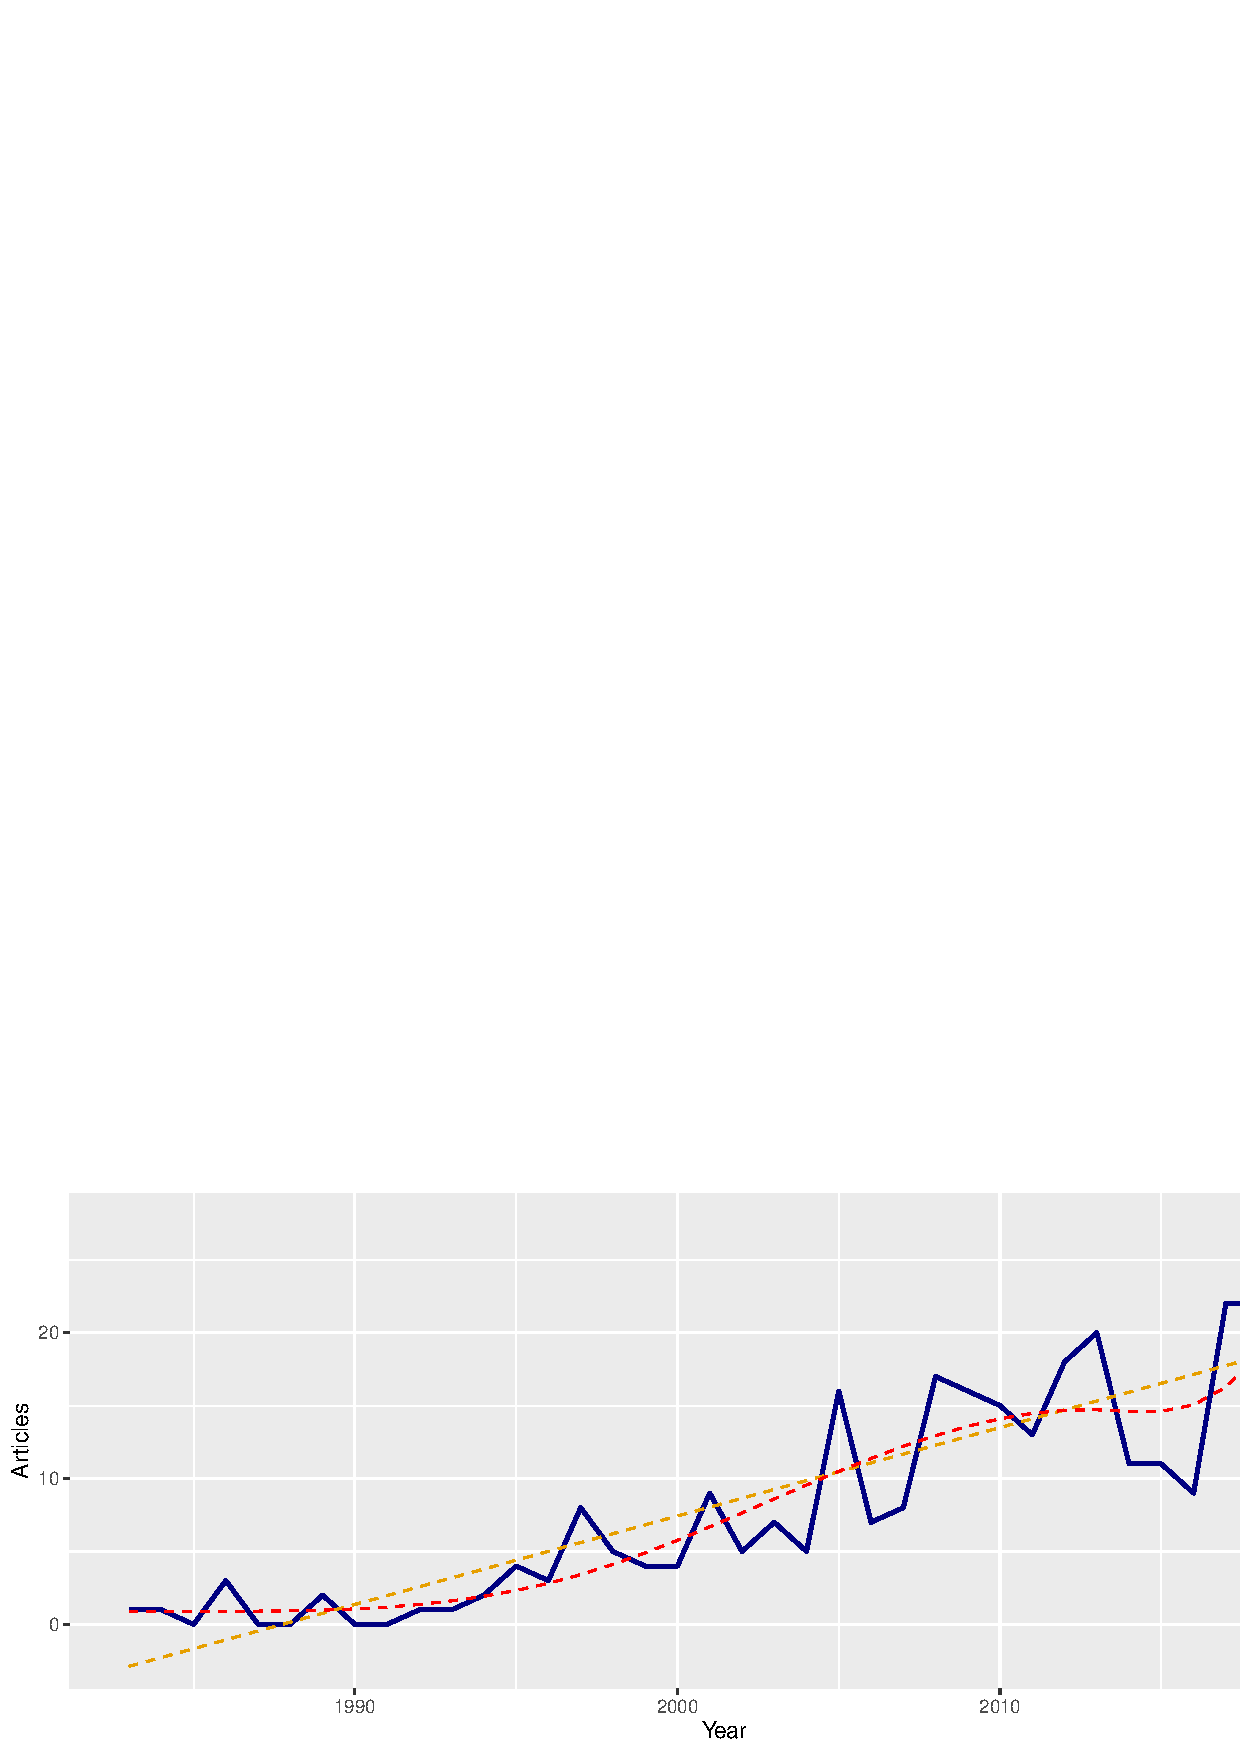
\includegraphics[width=0.9\textwidth]{Imagen1.JPEG}
\end{center}
\end{figure}

\end{frame}


%%%%%%%%%%%%%%%%%%%%%%%%%%%%%%%%%%%%%%%%%%%%%%%%%%%%%%%%%%%%


\begin{frame}[fragile]
\frametitle{Ejercicio}


Sobre la serie de precios de cierre diario de las acciones de Google. Aplique los métodos no estacionales: Promedio, Ingenuo, Deriva, para un horizonte de 40 observaciones. Realice el gráfico.

\vspace{4mm}
Sobre la serie auscafe aplique los cuatro métodos.

\vspace{6mm}

\lstset{language=r,label= ,caption= ,captionpos=b,numbers=none}
\begin{lstlisting}
goog200

auscafe
\end{lstlisting}



\end{frame}


%%%%%%%%%%%%%%%%%%%%%%%%%%%%%%%%%%%%%%%%%%%%%%%%%%%%%%%%%%%%


\begin{frame}[fragile]
\frametitle{Ejercicio}


\begin{figure}
\begin{center}
    \includegraphics[width=0.9\textwidth]{Imagen2.JPEG}
\end{center}
\end{figure}

\small{Cualquier método de pronóstico que desarrollemos se comparará con estos métodos simples para garantizar que el nuevo método sea mejor que estas alternativas simples. \highlighton{Si no, no vale la pena considerar el nuevo método.}
}
\end{frame}


%%%%%%%%%%%%%%%%%%%%%%%%%%%%%%%%%%%%%%%%%%%%%%%%%%%%%%%%%%%%



\section{Transformaciones}


\begin{frame}[fragile]
\frametitle{Transformaciones matemáticas}

Si los datos muestran variaciones que aumentan o disminuyen con el nivel de la serie, entonces una transformación puede ser útil.


\vspace{4mm}
\pause

\begin{itemize}
\item Si denotamos las observaciones originales como $y_1, ..., y_n$ y las observaciones transformadas como $w_1, ..., w_n$
\end{itemize}

\vspace{3mm}
\pause


\begin{block}{Trans. matemáticas para estabilizar la varianza}

\begin{itemize}
\item Raíz cuadrada: \hspace{5mm} $w_t = \sqrt{y_t}$
\item Raíz cúbica: \hspace{8mm} $w_t = \sqrt[3]{y_t}$
\item Logaritmo: \hspace{10mm} $w_t = log(y_t)$
\end{itemize}


\end{block}

\vspace{4mm}
\pause

{\small \highlighton{Los logaritmos, en particular, son útiles porque son más interpretables: los cambios en un valor de registro son cambios relativos (porcentaje) en la escala original.}
}

\end{frame}


%%%%%%%%%%%%%%%%%%%%%%%%%%%%%%%%%%%%%%%%%%%%%%%%%%%%%%%%%%%%



\begin{frame}[fragile]
\frametitle{Transformaciones matemáticas}


\begin{figure}
\begin{center}
    \includegraphics[width=0.8\textwidth]{Imagen4.JPG}
\end{center}
\end{figure}


\end{frame}


%%%%%%%%%%%%%%%%%%%%%%%%%%%%%%%%%%%%%%%%%%%%%%%%%%%%%%%%%%%%


\begin{frame}[fragile]
\frametitle{Transformaciones matemáticas}


\begin{figure}
\begin{center}
    \includegraphics[width=0.8\textwidth]{Imagen5.JPG}
\end{center}
\end{figure}


\end{frame}


%%%%%%%%%%%%%%%%%%%%%%%%%%%%%%%%%%%%%%%%%%%%%%%%%%%%%%%%%%%%



\begin{frame}[fragile]
\frametitle{Transformaciones matemáticas}


\begin{figure}
\begin{center}
    \includegraphics[width=0.8\textwidth]{Imagen6.JPG}
\end{center}
\end{figure}


\end{frame}


%%%%%%%%%%%%%%%%%%%%%%%%%%%%%%%%%%%%%%%%%%%%%%%%%%%%%%%%%%%%



\begin{frame}[fragile]
\frametitle{Transformaciones matemáticas}


\begin{figure}
\begin{center}
    \includegraphics[width=0.8\textwidth]{Imagen7.JPG}
\end{center}
\end{figure}


\end{frame}


%%%%%%%%%%%%%%%%%%%%%%%%%%%%%%%%%%%%%%%%%%%%%%%%%%%%%%%%%%%%



\begin{frame}
\frametitle{Transformación Box-Cox}

Una familia útil de transformaciones, que incluye tanto logaritmos como transformaciones de potencia, es la familia de las transformaciones de Box-Cox, que dependen del parámetro $\lambda$ y se definen de la siguiente manera:


\begin{equation}
w_t = 
   \begin{cases} 
      log(y_t)              & \lambda = 0   \\
      (y_t^\lambda -1) / \lambda & \mbox{otro caso}
   \end{cases}
\end{equation}

\pause

\begin{itemize}
\small
\item $\lambda = 0$ (Logaritmos naturales)
\item $\lambda = 1 \longrightarrow w_t = y_t - 1$ (los datos transformados se desplazan una unidad, pero no hay cambios en la serie de tiempo)
\item $\lambda = 1/2$ (Raíz cuadrada)
\item $\lambda = -1$ (Inversa)
\end{itemize}

{\small
\begin{center}
\highlighton{Un buen valor de $\lambda$ es el que hace que el tamaño de la variación estacional sea casi igual en toda la serie, ya que eso simplifica el modelo de pronóstico.}
\end{center}
}
\end{frame}


%%%%%%%%%%%%%%%%%%%%%%%%%%%%%%%%%%%%%%%%%%%%%%%%%%%%%%%%%%%%





\begin{frame}[fragile]
\frametitle{Transformación Box-Cox}

\textbf{Determine un buen valor para $\lambda$}

\lstset{language=r,label= ,caption= ,captionpos=b,numbers=none}
\begin{lstlisting}
p1<-list()

lambda <- seq(1, -1, by=-0.25)
for(i in seq_along(lambda)){
  p1[[i]]<-autoplot(BoxCox(elec,lambda[i])) + xlab("Year") +
          ylab("") +
          ggtitle(
            (paste("Transformed Australian electricity demand:  
                      lambda =",format(lambda[i],digits=2,nsmall=2))
          ))
      }

p1
\end{lstlisting}



\end{frame}


%%%%%%%%%%%%%%%%%%%%%%%%%%%%%%%%%%%%%%%%%%%%%%%%%%%%%%%%%%%%





\begin{frame}[fragile]
\frametitle{Transformación Box-Cox}

\textbf{Determine un buen valor para $\lambda$}

\vspace{4mm}

En este caso, $\lambda = 0.25$ funciona bastante bien, aunque cualquier valor de $\lambda$  entre 0 y 0.5 daría resultados similares.

\vspace{4mm}

La función \highlighton{BoxCox.lambda()} elegirá un valor de $\lambda$ para usted.

\begin{block}{BoxCox.lambda()}

\begin{lstlisting}
lambda <- BoxCox.lambda(elec)

[1] 0.2654

autoplot(BoxCox(elec,lambda))
\end{lstlisting}

\end{block}


\end{frame}


%%%%%%%%%%%%%%%%%%%%%%%%%%%%%%%%%%%%%%%%%%%%%%%%%%%%%%%%%%%%





\begin{frame}[fragile]
\frametitle{Transformación Box-Cox}

\begin{lstlisting}
lambda <- BoxCox.lambda(elec)

[1] 0.2654

autoplot(BoxCox(elec,lambda))
\end{lstlisting}


\begin{figure}
\begin{center}
    \includegraphics[width=0.8\textwidth]{Imagen8.JPG}
\end{center}
\end{figure}

\end{frame}


%%%%%%%%%%%%%%%%%%%%%%%%%%%%%%%%%%%%%%%%%%%%%%%%%%%%%%%%%%%%






\begin{frame}[fragile]
\frametitle{Transformación Box-Cox}

\begin{itemize}
\item Si algún $y_t = 0$, entonces debe tener $\lambda > 0$
\item si algún $y_t < 0$, no es posible la transformación de potencia a menos que todos los $y_t$ se ajusten agregando una constante a todos los valores
\item Los valores simples de $\lambda$ son más fáciles de explicar
\item Los resultados del pronóstico son relativamente insensibles a $\lambda$
\item Elegir $ \lambda = 0$ es una manera simple de forzar los pronósticos para que sean positivos
\item Las transformaciones a veces hacen poca diferencia en los pronósticos, pero tienen un gran efecto en los intervalos de predicción.
\end{itemize}



\end{frame}


%%%%%%%%%%%%%%%%%%%%%%%%%%%%%%%%%%%%%%%%%%%%%%%%%%%%%%%%%%%%




\begin{frame}
\frametitle{Transformación Box-Cox}

Habiendo elegido una transformación, necesitamos pronosticar los datos transformados. Entonces, tenemos que revertir la transformación (Back-transformation) para obtener predicciones en la escala original. La transformación inversa de Box-Cox viene dada por:

\vspace{4mm}

\begin{equation}
w_t = 
   \begin{cases} 
      exp(w_t)              & \lambda = 0   \\
      (\lambda w_t +1)^{1/\lambda}   & \mbox{otro caso}
   \end{cases}
\end{equation}


\end{frame}


%%%%%%%%%%%%%%%%%%%%%%%%%%%%%%%%%%%%%%%%%%%%%%%%%%%%%%%%%%%%



\begin{frame}[fragile]
\frametitle{Back-transformation}


\begin{lstlisting}
fit <- snaive(elec, lambda=1/3)
autoplot(fit)
\end{lstlisting}

\pause


\begin{figure}
\begin{center}
    \includegraphics[width=0.8\textwidth]{Imagen9.JPG}
\end{center}
\end{figure}


\end{frame}


%%%%%%%%%%%%%%%%%%%%%%%%%%%%%%%%%%%%%%%%%%%%%%%%%%%%%%%%%%%%




\begin{frame}[fragile]
\frametitle{Back-transformation}


\begin{lstlisting}
autoplot(fit, include=120)
\end{lstlisting}

\pause


\begin{figure}
\begin{center}
    \includegraphics[width=0.8\textwidth]{Imagen10.JPG}
\end{center}
\end{figure}


\end{frame}


%%%%%%%%%%%%%%%%%%%%%%%%%%%%%%%%%%%%%%%%%%%%%%%%%%%%%%%%%%%%



\section{Diagnóstico residual}
\begin{frame}
\frametitle{Valores ajustados}

Cada observación en una serie de tiempo puede pronosticarse utilizando todas las observaciones anteriores.

\vspace{4mm}

\begin{itemize}

\item Los llamamos valores ajustados y se denotan por \highlighton{$\hat{y}_{t|t-1}$}, lo cual significa que el pronóstico de $y_t$ está basado en las observaciones \highlighton{$y_1, ..., y_{t-1}$}.


\item Los usamos tan a menudo que a veces descartamos parte del subíndice y simplemente escribimos \highlighton{$\hat{y}_t \equiv \hat{y}_{t|t-1}$}

\end{itemize}


\begin{block}{Por ejemplo:}

\begin{itemize}
\item $\hat{y}_t = \bar{y}$ (método de la media)
\item $\hat{y}_t = y_{t-1} + (y_T - y_1)/(T-1)$ (método de la deriva)

\end{itemize}

\end{block}


\end{frame}


%%%%%%%%%%%%%%%%%%%%%%%%%%%%%%%%%%%%%%%%%%%%%%%%%%%%%%%%%%%%




\begin{frame}
\frametitle{Residuales en los pronósticos}

\begin{block}{}
Es el resultado de la diferencia entre los valores observados y los valores ajustados:

\begin{equation}
e_t = y_t - \hat{y}_{t|t-1}
\end{equation}

\end{block}


\vspace{4mm}


Un buen método de pronóstico arrojará residuos con las siguientes propiedades:

\begin{itemize}

\item Los residuos \highlighton{no están correlacionados}. Si hay correlaciones entre los residuos, entonces queda información en los residuos que debe usarse para calcular pronósticos. 


\item Los residuos tienen \highlighton{media cero}. Si los residuos tienen una media distinta de cero, entonces los pronósticos están sesgados.

\end{itemize}


\end{frame}


%%%%%%%%%%%%%%%%%%%%%%%%%%%%%%%%%%%%%%%%%%%%%%%%%%%%%%%%%%%%





\begin{frame}
\frametitle{Residuales en los pronósticos}

Además de las propiedades esenciales, es útil (pero no necesario) que los residuos también tengan las siguientes dos propiedades.:

\vspace{4mm}

\begin{itemize}

\item Los residuos tienen varianza constante.

\item Los residuos se distribuyen normalmente.

\end{itemize}

\vspace{4mm}

Estas dos propiedades facilitan el cálculo de los intervalos de predicción. Si no se cumple, es necesario un enfoque alternativo para obtener intervalos de predicción.

\end{frame}


%%%%%%%%%%%%%%%%%%%%%%%%%%%%%%%%%%%%%%%%%%%%%%%%%%%%%%%%%%%%





\begin{frame}[fragile]
\frametitle{Ejemplo}


\begin{lstlisting}
autoplot(goog200) +
xlab("Day") + ylab("Closing Price (US$)") +
ggtitle("Google Stock (daily ending 6 December 2013)")
\end{lstlisting}

\pause


\begin{figure}
\begin{center}
    \includegraphics[width=0.8\textwidth]{Imagen11.JPG}
\end{center}
\end{figure}


\end{frame}


%%%%%%%%%%%%%%%%%%%%%%%%%%%%%%%%%%%%%%%%%%%%%%%%%%%%%%%%%%%%


\begin{frame}[fragile]
\frametitle{Ejemplo}


\begin{itemize}
\item El anterior gráfico muestra el precio de cierre de acciones diario de Google. El gran salto en el día 166 corresponde al 18 de octubre de 2013, cuando el precio subió un 12\% debido a resultados inesperadamente fuertes del tercer trimestre.

\vspace{3mm}

\item Para los precios e índices del mercado de valores, el mejor método de pronóstico es a menudo el método ingenuo. Es decir, cada pronóstico es simplemente igual al último valor observado: \highlighton{$\hat{y}_t = y_{t|t-1}$}

\vspace{3mm}

\item Por lo tanto, los residuos son simplemente iguales a la diferencia entre observaciones consecutivas:

\begin{equation}
\highlighton{e_t = y_t - \hat{y}_t = y_t - y_{t-1}}
\end{equation}


\end{itemize}

\end{frame}


%%%%%%%%%%%%%%%%%%%%%%%%%%%%%%%%%%%%%%%%%%%%%%%%%%%%%%%%%%%%




\begin{frame}[fragile]
\frametitle{Ejemplo}


\begin{lstlisting}
fits <- fitted(naive(goog200))
autoplot(goog200, series="Data") +
autolayer(fits, series="Fitted") +
xlab("Day") + ylab("Closing Price (US$)") +
ggtitle("Google Stock (daily ending 6 December 2013)")
\end{lstlisting}

\pause


\begin{figure}
\begin{center}
    \includegraphics[width=0.8\textwidth]{Imagen12.JPG}
\end{center}
\end{figure}


\end{frame}


%%%%%%%%%%%%%%%%%%%%%%%%%%%%%%%%%%%%%%%%%%%%%%%%%%%%%%%%%%%%





\begin{frame}[fragile]
\frametitle{Ejemplo}


\begin{lstlisting}
res <- residuals(naive(goog200))
autoplot(res) + xlab("Day") + ylab("") +
  ggtitle("Residuals from naive method")
\end{lstlisting}

\pause


\begin{figure}
\begin{center}
    \includegraphics[width=0.8\textwidth]{Imagen13.JPG}
\end{center}
\end{figure}


\end{frame}


%%%%%%%%%%%%%%%%%%%%%%%%%%%%%%%%%%%%%%%%%%%%%%%%%%%%%%%%%%%%




\begin{frame}[fragile]
\frametitle{Ejemplo}


\begin{lstlisting}
gghistogram(res, add.normal=TRUE) +
ggtitle("Histogram of residuals")
\end{lstlisting}

\pause


\begin{figure}
\begin{center}
    \includegraphics[width=0.8\textwidth]{Imagen14.JPG}
\end{center}
\end{figure}


\end{frame}


%%%%%%%%%%%%%%%%%%%%%%%%%%%%%%%%%%%%%%%%%%%%%%%%%%%%%%%%%%%%




\begin{frame}[fragile]
\frametitle{Ejemplo}


\begin{lstlisting}
gghistogram(res, add.normal=TRUE) +
ggtitle("Histogram of residuals")
\end{lstlisting}

\pause


\begin{figure}
\begin{center}
    \includegraphics[width=0.8\textwidth]{Imagen15.JPG}
\end{center}
\end{figure}


\end{frame}


%%%%%%%%%%%%%%%%%%%%%%%%%%%%%%%%%%%%%%%%%%%%%%%%%%%%%%%%%%%%





\begin{frame}[fragile]
\frametitle{Ejemplo}


\begin{itemize}
\small
\item Estos gráficos muestran que el método ingenuo produce pronósticos que parecen dar cuenta de toda la información disponible.

\item \highlighton{La media de los residuos es cercana a cero y no existe una correlación significativa en la serie de residuos.}

\item El gráfico de tiempo de los residuos muestra que la variación de los residuos se mantiene casi igual en los datos históricos, aparte del valor atípico, y por lo tanto, la variación residual puede tratarse como constante.

\item \highlighton{El histograma sugiere que los residuos pueden no ser normales: la cola derecha parece demasiado larga, incluso si ignoramos el valor atípico. }
\end{itemize}

\vspace{4mm}

\begin{center}
Los pronósticos de este método probablemente serán bastante buenos, pero los \textcolor{blue}{intervalos de predicción} que se calculan suponiendo una distribución normal pueden ser \textcolor{blue}{inexactos}.

\end{center}
\end{frame}


%%%%%%%%%%%%%%%%%%%%%%%%%%%%%%%%%%%%%%%%%%%%%%%%%%%%%%%%%%%%


\begin{frame}
\frametitle{Prueba de Portmanteau}

Además de mirar el diagrama de ACF, también podemos hacer una prueba más formal para la autocorrelación considerando un conjunto completo de valores  \highlighton{$r_k$} como un grupo, en lugar de tratar a cada uno por separado. \textcolor{red}{Recordemos que $r_k$ es la autocorrelación para el rezago $k$.}
  
\begin{block}{Prueba Box-Pierce}

\begin{equation}
Q = T \sum_{k=1}^{h} r_k^2
\end{equation}

dónde $h$ es el máximo rezago que se esta considerando y $T$ es el número de observaciones.

\end{block} 

\pause

\begin{itemize}
\item Si cada $r_k$ está cerca de cero, entonces $Q$ será pequeño.
\item Si algunos valores de $r_k$ son grandes (positivos o negativos), $Q$ será grande.
\end{itemize}


\end{frame}


%%%%%%%%%%%%%%%%%%%%%%%%%%%%%%%%%%%%%%%%%%%%%%%%%%%%%%%%%%%%





\begin{frame}
\frametitle{Prueba de Portmanteau}

Además de mirar el diagrama de ACF, también podemos hacer una prueba más formal para la autocorrelación considerando un conjunto completo de valores  \highlighton{$r_k$} como un grupo, en lugar de tratar a cada uno por separado. \textcolor{red}{Recordemos que $r_k$ es la autocorrelación para el rezago $k$.}
  
\begin{block}{Prueba Ljung-Box (Una prueba más precisa)}

\begin{equation}
Q^* = T(T+2) \sum_{k=1}^{h}(T-k) r_k^2
\end{equation}

dónde $h$ es el máximo rezago que se esta considerando y $T$ es el número de observaciones.

\end{block} 

\pause

\begin{itemize}
\item Recomendación: $h = 10$ para datos no estacionales. $h = 2m$ para datos estacionales, donde $m$ es el periodo de estacionalidad.
\item Mejor rendimiento, especialmente en muestras pequeñas.
\end{itemize}


\end{frame}


%%%%%%%%%%%%%%%%%%%%%%%%%%%%%%%%%%%%%%%%%%%%%%%%%%%%%%%%%%%%


\begin{frame}
\frametitle{Prueba Portmanteau}

\highlighton{Grandes valores de $Q^*$ sugieren que las autocorrelaciones no provienen de una serie de ruido blanco.} 

\vspace{3mm}

¿Qué tan grande es demasiado grande? 

\begin{itemize}
\item Si las autocorrelaciones vinieron de una serie de ruido blanco, entonces ambas $Q$ y $Q^*$ tendría una distribución $\chi^2$ con $(h - k)$ grados de libertad, dónde $k$ es el número de parámetros en el modelo.

\vspace{4mm}

\item Si se calculan a partir de datos sin procesar (en lugar de los residuos de un modelo), establezca $k=0$

\end{itemize}


\end{frame}


%%%%%%%%%%%%%%%%%%%%%%%%%%%%%%%%%%%%%%%%%%%%%%%%%%%%%%%%%%%%




\begin{frame}[fragile]
\frametitle{Prueba Portmanteau}

Para el ejemplo del precio de las acciones de Google, el modelo ingenuo no tiene parámetros, por lo que $K= 0$, en ese caso también.

\vspace{4mm}


\begin{lstlisting}
# lag=h and fitdf=K
Box.test(res, lag=10, fitdf=0)
\end{lstlisting}

\pause

{\small
\begin{verbatim}
Box-Pierce test

data:  res
X-squared = 10.611, df = 10, p-value = 0.3886
\end{verbatim}
}

\pause


\begin{lstlisting}
Box.test(res,lag=10, fitdf=0, type="Lj")
\end{lstlisting}

\pause

{\small
\begin{verbatim}
Box-Ljung test

data:  res
X-squared = 11.031, df = 10, p-value = 0.3551
\end{verbatim}
}

\end{frame}


%%%%%%%%%%%%%%%%%%%%%%%%%%%%%%%%%%%%%%%%%%%%%%%%%%%%%%%%%%%%




\begin{frame}[fragile]
\frametitle{Prueba Portmanteau}



\begin{lstlisting}
checkresiduals(naive(goog200))
\end{lstlisting}

\pause

\begin{figure}
\begin{center}
    \includegraphics[width=0.8\textwidth]{Imagen16.JPG}
\end{center}
\end{figure}

\end{frame}


%%%%%%%%%%%%%%%%%%%%%%%%%%%%%%%%%%%%%%%%%%%%%%%%%%%%%%%%%%%%




\begin{frame}[fragile]
\frametitle{Prueba Portmanteau}



\begin{lstlisting}
checkresiduals(naive(goog200))
\end{lstlisting}



\begin{verbatim}
Ljung-Box test

data:  Residuals from Naive method
Q* = 11.031, df = 10, p-value = 0.3551

Model df: 0.   Total lags used: 10
\end{verbatim}

\end{frame}


%%%%%%%%%%%%%%%%%%%%%%%%%%%%%%%%%%%%%%%%%%%%%%%%%%%%%%%%%%%%




%%%%%%%%%%%%%%%%%%%%%%%%%%%%%%%%%%%%%%%%%%%%%%%%%%%%%%%%%%%%








%%%%%%%%%%%%%%%%%%%%%%%%%%%%%%%%%%%%%%%%%%%%%%%%%%%%%%%%%%%%%%%%%%%%%%%











%%%%%%%%%%%%%%%%%%%%%%%%%%%%%%%%%%%%%%%%%%%%%%%%%%%%%%%%%%%%%%%%%%%%% 




\frame{
  \vspace{2cm}
  {\huge Preguntas?}


\vspace{2.5cm}

\begin{flushright}
\highlighton{
  \usebeamerfont*{frametitle}Gracias!!},
\end{flushright}

  
  \begin{flushright}
    Jr.
    
   \structure{\footnotesize{orlando.joaqui@correounivalle.edu.co}}
  \end{flushright}
}







\end{document}
